\documentclass[12pt]{article}

\title{Activity 12: Arrays of Objects}
\author{Dr. Chris Mayfield}
\date{CS 149, Fall 2016}

%\ProvidesPackage{cspogil}

% fonts
\usepackage[utf8]{inputenc}
\usepackage[T1]{fontenc}
\usepackage{mathpazo}

% spacing
\usepackage[margin=2cm]{geometry}
\renewcommand{\arraystretch}{1.4}
\setlength{\parindent}{0pt}

% orphans and widows
\clubpenalty=10000
\widowpenalty=10000
\pagestyle{empty}

% figures and tables
\usepackage{graphicx}
\usepackage{multicol}
\usepackage{tabularx}
\usepackage{wrapfig}

% fixed-width columns
\usepackage{array}
\newcolumntype{L}[1]{>{\raggedright\let\newline\\\arraybackslash\hspace{0pt}}m{#1}}
\newcolumntype{C}[1]{>{\centering\let\newline\\\arraybackslash\hspace{0pt}}m{#1}}
\newcolumntype{R}[1]{>{\raggedleft\let\newline\\\arraybackslash\hspace{0pt}}m{#1}}

% include paths
\makeatletter
\def\input@path{{Models/}{../../Models/}}
\graphicspath{{Models/}{../../Models/}}
\makeatother

% colors
\usepackage[svgnames,table]{xcolor}
\definecolor{bgcolor}{HTML}{FAFAFA}
\definecolor{comment}{HTML}{007C00}
\definecolor{keyword}{HTML}{0000FF}
\definecolor{strings}{HTML}{B20000}

% table headers
\newcommand{\tr}{\bf\cellcolor{Yellow!10}}

% syntax highlighting
\usepackage{textcomp}
\usepackage{listings}
\lstset{
    basicstyle=\ttfamily\color{black},
    backgroundcolor=\color{bgcolor},
    numberstyle=\scriptsize\color{comment},
    commentstyle=\color{comment},
    keywordstyle=\color{keyword},
    stringstyle=\color{strings},
    columns=fullflexible,
    keepspaces=true,
    showlines=true,
    showstringspaces=false,
    upquote=true
}

% code environments
\newcommand{\java}[1]{\lstinline[language=java]{#1}}%[
\lstnewenvironment{javalst}{\lstset{language=java,backgroundcolor=}}{}
\lstnewenvironment{javabox}{\lstset{language=java,frame=single,numbers=left}\quote}{\endquote}

% PDF properties
\usepackage[pdftex]{hyperref}
\urlstyle{same}
\makeatletter
\hypersetup{
  pdftitle={\@title},
  pdfauthor={\@author},
  pdfsubject={\@date},
  pdfkeywords={},
  bookmarksopen=false,
  colorlinks=true,
  citecolor=black,
  filecolor=black,
  linkcolor=black,
  urlcolor=blue
}
\makeatother

% titles
\makeatletter
\renewcommand{\maketitle}{\begin{center}\LARGE\@title\end{center}}
\makeatother

% boxes [optional height]
\newcommand{\emptybox}[1][10em]{
\vspace{1em}
\begin{tabularx}{\linewidth}{|X|}
\hline\\[#1]\hline
\end{tabularx}}

% models
\newcommand{\model}[1]{\section{#1}\nopagebreak}
\renewcommand{\thesection}{Model~\arabic{section}}

% questions
\newcommand{\quest}[1]{\subsection*{Questions~ (#1)}}
\newcounter{question}
\newcommand{\Q}{\vspace{1em}\refstepcounter{question}\arabic{question}.~ }
\renewcommand{\thequestion}{\#\arabic{question}}

% sub-question lists
\usepackage{enumitem}
\setenumerate[1]{label=\alph*)}
\setlist{itemsep=1em,after=\vspace{1ex}}

% inline answers
\definecolor{answers}{HTML}{C0C0C0}
\newcommand{\ans}[1]{%
\ifdefined\Student
    \leavevmode\phantom{~~\textcolor{answers}{#1}}
\else
    ~~\textcolor{answers}{#1}
\fi}

% longer answers [optional height]
\newsavebox{\ansbox}
\newenvironment{answer}[1][4em]{
\nopagebreak
\begin{lrbox}{\ansbox}
\begin{minipage}[t][#1]{\linewidth}
\color{answers}
}{
\end{minipage}
\end{lrbox}
\ifdefined\Student
    \phantom{\usebox{\ansbox}}%
\else
    \usebox{\ansbox}%
\fi}


\begin{document}

\maketitle

With arrays and objects, you can represent pretty much any type of data.
It's not only possible to have arrays of objects, but also objects of arrays, objects of objects, arrays of arrays, arrays of objects of arrays, and so forth.

\model{Yahtzee Dice}

Creating an array of objects is typically a 3-step process:

\begin{center}
%TODO where did this image come from? Ralph Grove?
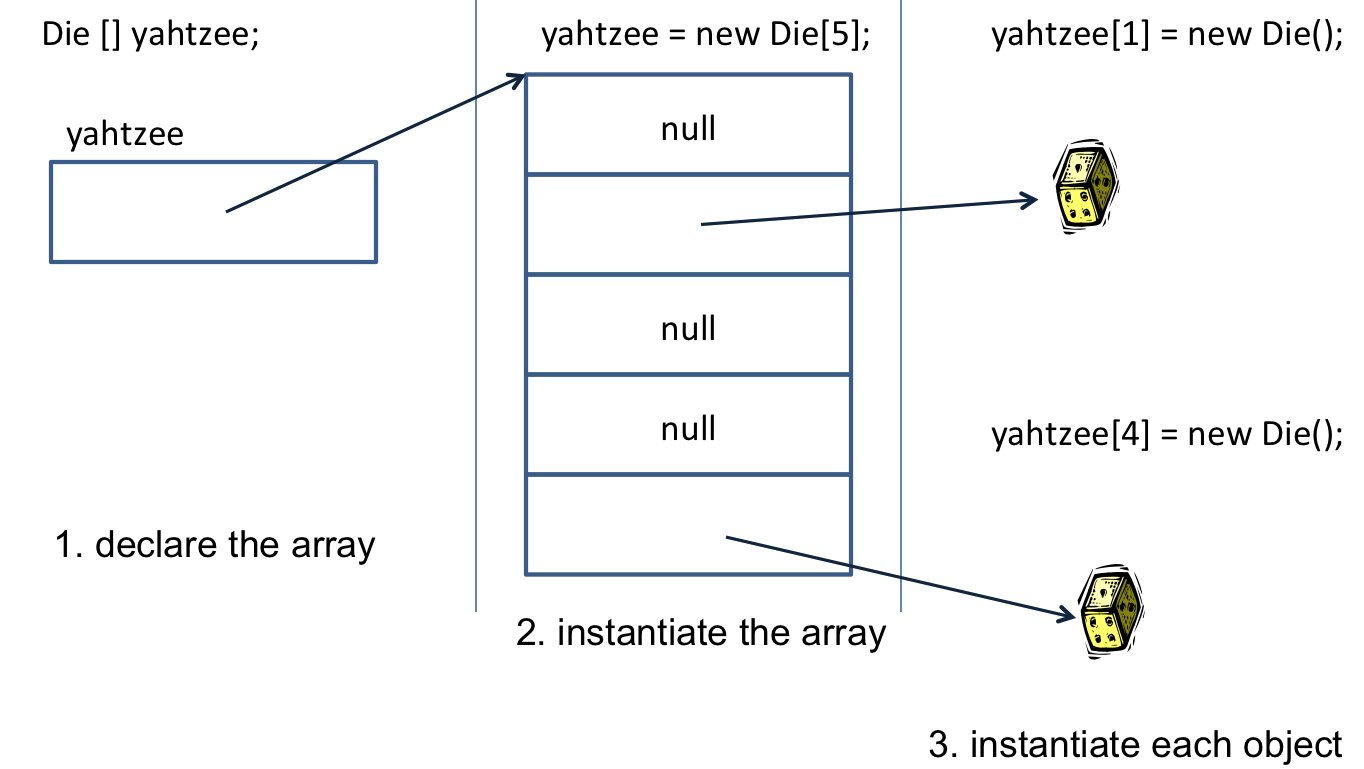
\includegraphics[width=5.5in]{CS1B/yahtzee-array.png}
\end{center}


\quest{15 min}


\Q What is the type of the local variable \java{yahtzee}?
What is its initial value? (Hint: it's not \java{null}.)

\begin{answer}
It's an array of \java{Die} objects. Until it's assigned for the first time, it's uninitialized (meaning you that can't read its value).
\end{answer}


\Q When you create an array (e.g., ~\java{new Die[5]}) what is the initial value of each element?

\begin{answer}
The initial values are automatically set to null (for reference types). For arrays of integers, it's 0; for doubles, it's 0.0; for booleans, it's {\tt false}; for characters, it's the unicode character \chr{\textbackslash u0000}.
\end{answer}


\Q When you construct a new object (e.g., ~\java{new Die()}) what are the initial values of its attributes (e.g., ~\java{this.face})?

\begin{answer}
All attributes are initialized to the value of ``zero'' for that data type.
So references are {\tt null}, integers are 0, doubles are 0.0, and so forth.
\end{answer}


\Q Describe in your own words what the following statement does. Be sure to explain how the random part works.

\begin{center}
\java{yahtzee[(int) (Math.random() * yahtzee.length)] = null;}
\end{center}

\begin{answer}
\java{Math.random()} returns a value in the range [0, 1).
Multiplying that value by \java{yahtzee.length} and then casting it to an integer gives a value in the range 0..5 inclusive.
So this statement randomly sets of the dice references to {\tt null}.
\end{answer}


\Q \label{fordie} What is the result of running the loop below?
What is the purpose of the nested if-statement?

\begin{javalst}
for (int i = 0; i < yahtzee.length; i++) {
    if (yahtzee[i] != null) {
        yahtzee[i].roll();
    }
}
\end{javalst}
\vspace{-1ex}

\begin{answer}
This loop rolls the dice in the array.
Because some of the dice are {\tt null}, the if-statement prevents {\tt NullPointerException}.
\end{answer}


\Q The enhanced for loop allows you to iterate the elements of an array.
Another name for this structure is the ``for each'' loop.
Rewrite the following example using a standard for loop.

\vspace{1ex}
\begin{javalst}
String[] days = {"Sun", "Mon", "Tue", "Wed", "Thu", "Fri", "Sat"};
for (String day : days) {
    System.out.println(day + " is a great day!");
}
\end{javalst}
\vspace{-1em}

\begin{answer}[5em]
\begin{javaans}
for (int i = 0; i < days.length; i++) {
    System.out.println(days[i] + " is a great day!");
}
\end{javaans}
\end{answer}


\Q In contrast to enhanced for loops, what does a standard for loop typically iterate?
Why would it be misleading to name the enhanced for loop variable \java{i} instead of \java{day}?

\begin{answer}
Standard for loops typically iterate indexes; that's why the variable is almost always named \java{i}.
\end{answer}


\Q Rewrite the loop in \ref{fordie} using an enhanced for loop.
Use an appropriate variable name for the \java{Die} object (i.e., not \java{i}).

\vspace{-1ex}
\begin{answer}[7em]
\begin{javaans}
for (Die die : yahtzee) {
    if (die != null) {
        die.roll();
    }
}
\end{javaans}
\end{answer}

\model{Deck of Cards}

There are 52 cards in a standard deck.
Each card belongs to one of four suits (Clubs, Diamonds, Hearts, and Spades) and one of 13 ranks (Ace, 2, 3, 4, 5, 6, 7, 8, 9, 10, Jack, Queen, and King).
The array below is one-dimensional, but the cards are displayed on four lines for convenience.

\begin{center}
% http://www.milefoot.com/math/discrete/counting/cardfreq.htm
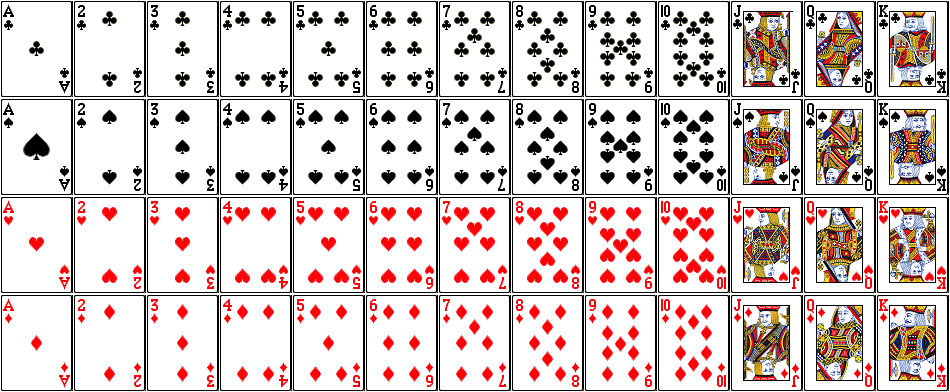
\includegraphics[width=\linewidth]{playing-cards1.png}
\end{center}


\quest{20 min}


\Q Implement the following constructor.
The class has two attributes: \java{rank} and \java{suit}.
Don't think too hard about it.

\begin{javalst}
/**
 * Constructs a face card given its rank and suit.
 *
 * @param rank face value (1 = ace, 11 = jack, 12 = queen, 13 = king)
 * @param suit category ("clubs", "diamonds", "hearts", or "spades")
 */
public Card(int rank, String suit) {
\end{javalst}

\vspace*{-1em}
\begin{answer}
\begin{javaans}
    this.rank = rank;
    this.suit = suit;
\end{javaans}
\end{answer}
\vspace*{-1em}

\begin{javalst}
}
\end{javalst}


\Q In one line of code, declare an array of strings named \java{suits} and initialize its contents to the four possible suits as shown above.

\vspace*{-1ex}
\begin{answer}
\begin{javaans}
    String[] suits = {"clubs", "spades", "hearts", "diamonds"};
\end{javaans}
\end{answer}


\Q Write several lines of code to declare and create an array of 52 \java{Card} objects.
Use nested \java{for} loops to construct \java{Card} objects in the order of the Model.
Make use of your \java{suits} array from the previous question.
Discuss with your team how you will keep track of the array index.

\vspace*{-1ex}
\begin{answer}[11em]
\begin{javaans}
Card[] cards = new Card[52];
int index = 0;
for (String suit : suits) {
    for (int rank = 1; rank <= 13; rank++) {
        cards[index] = new Card(rank, suit);
        index++;
    }
}
\end{javaans}
\end{answer}


\Q Describe what the following code does and how it works. (Note: You've come a long way this semester, to be able to understand this example!)

\begin{javalst}
public static Card[] sort(Card[] deck) {
    if (deck == null) {
        System.err.println("Missing deck!");
        return null;
    }
    Card[] sorted = new Card[deck.length];
    for (Card card : deck) {
        int index = card.position();       // returns suit * 13 + rank - 1
        sorted[index] = card;
    }
    return sorted;
}
\end{javalst}

\begin{answer}[5em]
This example sorts an array of cards.
It first validates the arguments, then it creates a new array of cards and assigns each \java{Card} reference according to its known position in the deck.
\end{answer}


\Q Write a static method named \java{inDeck} that takes a \java{Card[]} representing a deck of cards and a \java{Card} object representing a single card, and that returns \java{true} if the card is somewhere in the deck of cards. Be sure to use the equals method of the \java{Card} object to make comparisons.

\vspace{-1ex}
\begin{answer}[11em]
\begin{javaans}
public static boolean inDeck(Card[] deck, Card card) {
    for (Card c : deck) {
        if (c.equals(card)) {
            return true;
        }
    }
    return false;
}
\end{javaans}
\end{answer}


\end{document}
